% !TEX root = ../Preparazione alle olimpiadi.tex

\chapter{Strutture dati in C++}

\section{Vector}

Il \textbf{vector} è una struttura dati della Standard Template Library (STL) che rappresenta un \textbf{array dinamico}.  
A differenza degli array statici, la sua dimensione può crescere o ridursi durante l'esecuzione del programma.  
È contenitore sequenziale, quindi mantiene l'ordine degli elementi inseriti.



\textbf{Dichiarazione di un vector:}
\begin{lstlisting}[language=C++]
	#include <vector>
	#include <iostream>
	using namespace std;
	
	vector<int> v;            // vector vuoto di interi
	
	vector<int> v2(10);       // vector di 10 elementi 				inizializzati a 0
	
	vector<int> v3(5, 7);     // vector di 5 elementi inizializzati 						a 7
\end{lstlisting}


Prima di andare ai metodi di questa struttura, è opportuno spendere due parole sugli iteratori.

\subsection{Iterazione tramite \texttt{begin()} e \texttt{end()}}

I metodi \texttt{begin()} ed \texttt{end()} sono due funzioni fondamentali dei contenitori della STL, come \texttt{vector}, e servono per ottenere \textbf{iteratori} che consentono di scorrere gli elementi del contenitore.

\begin{itemize}
	\item \textbf{\texttt{v.begin()}}  
	Restituisce un iteratore che punta al \textbf{primo elemento} del \texttt{vector}.  
	È come un "puntatore" all'inizio della sequenza di dati.
	
	\item \textbf{\texttt{v.end()}}  
	Restituisce un iteratore che punta \textbf{alla posizione successiva all'ultimo elemento} del \texttt{vector}.  
	Non rappresenta quindi un elemento valido, ma serve per \textbf{indicare la fine} del contenitore.
\end{itemize}

L'uso tipico di \texttt{begin()} e \texttt{end()} è all'interno di un ciclo, per visitare tutti gli elementi del \texttt{vector}:

\newpage

\begin{lstlisting}[language=C++]
	#include <iostream>
	#include <vector>
	using namespace std;
	
	int main() {
		vector<int> v = {10, 20, 30, 40};
		
		for (auto it = v.begin(); it != v.end(); ++it) {
			cout << *it << " ";
		}
		return 0;
	}
\end{lstlisting}

In questo esempio:
\begin{itemize}
	\item \texttt{auto it = v.begin();} inizializza l'iteratore al primo elemento\footnote{È stato usato un \textbf{auto it} in quanto \textbf{it} viene confrontato con l'iteratore \textbf{v.end()} ed è opportuno che questi siano dello stesso tipo.} \footnote{In alternativa, avrei potuto usare \textbf{vector<int>::iterator it}};
	\item il ciclo prosegue finché \texttt{it} non raggiunge \texttt{v.end()}, cioè finché ci sono elementi validi;
	\item \texttt{*it} consente di accedere al valore dell'elemento puntato.
\end{itemize}

\textbf{Nota:}  
\texttt{v.end()} non punta a un elemento valido, quindi non bisogna mai dereferenziarlo (cioè non fare \texttt{*v.end()}), poiché ciò porterebbe a un comportamento indefinito.

\begin{figure}[h!]
	\centering
	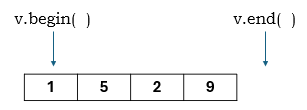
\includegraphics[width=0.4\textwidth]{immagini/2 - Strutture Dati/vector/vectoriteratori.png}
	\caption{Iteratori \textbf{v.begin()} e \textbf{v.end()}}
	\label{fig:strutture-dati:v.begin v.end}
\end{figure}




\subsection{Operazioni principali sui vector}
\begin{itemize}
	
		\item \textbf{Accesso agli elementi:} \texttt{v[i]}
	\begin{lstlisting}[language=C++]
		int x = v[1];     // accesso diretto 				(senza controllo)
		cout << x;	  //stampa l'elemento di v all'			indice 1
		
	\end{lstlisting}
	Complessità: O(1).
	
	
	\begin{figure}[h!]
		\centering
		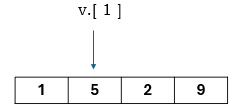
\includegraphics[width=0.3\textwidth]{immagini/2 - Strutture Dati/vector/vectoraccesso.png}
		\caption{Accesso ad un elemento del vettore}
		\label{fig:strutture-dati:v[1]}
	\end{figure}
	
	
	\item \textbf{Aggiunta in coda:} \texttt{push\_back(x)}
	\begin{lstlisting}[language=C++]
		v.push_back(3); // aggiunge 3 alla fine
	\end{lstlisting}
	Complessità: O(1).
	
	\begin{figure}[h!]
		\centering
		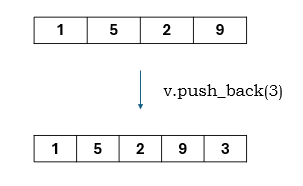
\includegraphics[width=0.3\textwidth]{immagini/2 - Strutture Dati/vector/vectorpushback.png}
		\caption{Inserimento di un elemento alla fine del vector}
		\label{fig:strutture-dati:v.push_back}
	\end{figure}
	
	
	
	
	
	\newpage
	
	\item \textbf{Rimozione dall'ultima posizione:} \texttt{pop\_back()}
	\begin{lstlisting}[language=C++]
		v.pop_back(); // rimuove l'ultimo elemento
	\end{lstlisting}
	Complessità: O(1).
	
	
	\begin{figure}[h!]
		\centering
		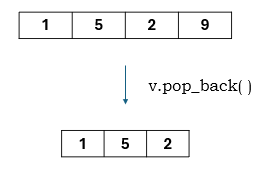
\includegraphics[width=0.3\textwidth]{immagini/2 - Strutture Dati/vector/vectorpopback.png}
		\caption{Cancellazione dell'ultimo elemento del vettore}
		\label{fig:strutture-dati:v.pop_back}
	\end{figure}
	
	
	
	
	

	
	
	
	
	
	\item \textbf{Dimensione:} \texttt{v.size()}  
	Restituisce il numero di elementi presenti nel vector.
	
	\begin{figure}[h!]
		\centering
		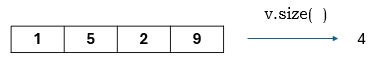
\includegraphics[width=0.45\textwidth]{immagini/2 - Strutture Dati/vector/vectorsize.png}
		\caption{Numero di elementi nel vettore}
		\label{fig:strutture-dati:v.size}
	\end{figure}
	
	\item \textbf{Controllo se vuoto:} \texttt{v.empty()}  
	Restituisce \texttt{true} se il vector non contiene elementi.
\end{itemize}

\subsection{Inserimento ed eliminazione in posizioni specifiche}
\begin{lstlisting}[language=C++]
	v.insert(v.begin() + 2, 10); // inserisce 10 in posizione 2 e 							shifta a destra tutti gli altri elementi
	
	v.erase(v.begin() + 2);      // elimina elemento in posizione 2 e 							shifta a sinistra tutti gli altri 							elementi
\end{lstlisting}

\textbf{Note: }

\begin{itemize}
	\item Inserimenti o cancellazioni in mezzo al vector hanno complessità O(n), perché gli elementi successivi devono essere spostati.
	
	
\end{itemize}



\subsection{Altre operazioni utili}
\begin{itemize}
	\item \texttt{v.clear()} → svuota il vector, O(n)
	\item \texttt{v.front()} → accede al primo elemento, O(1)
	\item \texttt{v.back()} → accede all'ultimo elemento, O(1)
	\item \texttt{v.resize(k)} → cambia la dimensione a k elementi (elimina quelli di troppo)
	
\end{itemize}



\subsection{Iterazione su un vector}
\begin{lstlisting}[language=C++]
	// Utilizzo di un ciclo for tradizionale
	for (size_t i = 0; i < v.size(); i++) {
		cout << v[i] << " ";
	}
	
	// Utilizzo del range-based for (C++11+)
	for (int x : v) {
		cout << x << " ";
	}
	
	// Utilizzo di iteratori
	for (vector<int>::iterator it = v.begin(); it != v.end(); ++it) {
		cout << *it << " ";
	}
\end{lstlisting}

\textbf{Note: }

\begin{itemize}
	\item la variabile di controllo del \texttt{for} è stata dichiarata come tipo \textbf{size\_t}. Questo perché verrà confrontata con \textbf{v.size()} che, di fatto, è anch'essa di tipo \textbf{size\_t}.
	\item \textbf{int x : v} è una sintassi valida da C++11 in poi. Molto semplicemente, \textbf{x} assume il valore di ogni elemento del vector \textbf{v}.
	In altre parole \textbf{x} è una copia e, come tale, non fa cambiare il valore degli elementi di \textbf{v} in caso scrivessi \textbf{x = 2}.
\end{itemize}



\newpage

\subsection{Complessità computazionale riassunta}

\begin{table}[h!]
	\centering
	\renewcommand{\arraystretch}{1.5}
	\setlength{\tabcolsep}{12pt}
	\begin{tabular}{|c|c|}
		\hline
		\textbf{Operazione} & \textbf{Complessità} \\
		\hline
		\makecell{Accesso a un elemento \\ \texttt{v[i]}} & O(1) \\
		\hline
		\makecell{Inserimento in mezzo \\ \texttt{v.insert(iteratore, valore)}} & O(n) \\
		\hline
		\makecell{Cancellazione in mezzo \\ \texttt{v.erase(iteratore)}} & O(n) \\
		\hline
		\makecell{	Aggiunta in coda \\ \texttt{v.push\_back(valore)}} & O(1) \\
		\hline
		\makecell{Eliminazione ultimo elemento \texttt{v.pop\_back()}} & O(1) \\
		\hline
		\makecell{Dimensione \texttt{v.size()}} & O(1) \\
		\hline
		
	\end{tabular}
	\caption{Complessità operazioni principali sui vector}
\end{table}

\newpage




\section{Map}

La \textbf{map} è una struttura dati della Standard Template Library (STL) che rappresenta un \textbf{contenitore associativo ordinato}.  
Permette di memorizzare coppie chiave-valore e garantisce che le chiavi siano \textbf{uniche} e \textbf{automaticamente ordinate}.
Per accedere al valore, quindi, ho bisogno della chiave.

In figura \ref{fig:strutture-dati:map} si può notare come le chiavi (\texttt{int}) siano ordinate in ordine crescente e siano associate a dei valori (\texttt{string})

\begin{figure}[h!]
	\centering
	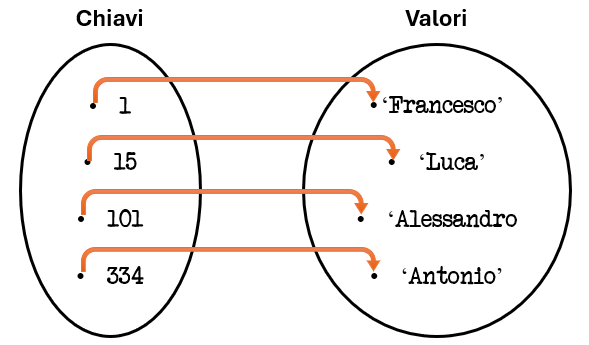
\includegraphics[width=0.6\textwidth]{immagini/2 - Strutture Dati/map/map.png}
	\caption{Rappresentazione grafica di una \textbf{map}}
	\label{fig:strutture-dati:map}
\end{figure}

\subsection{Dichiarazione di una map}

\begin{lstlisting}[language=C++]
	#include <map>
	#include <iostream>
	using namespace std;
	
	map<string, int> m1;           // mappa con chiavi stringa e valori interi
	
	map<int, string> m2 = {        // mappa inizializzata con le coppie 							chiave-valore (le coppie saranno 							ordinate in ordine di chiave 								crescente automaticamente) 
		{101, "Alessandro"},
		{334, "Antonio"},
		{1, "Francesco"},
		{15 ,"Luca"}
	};
	
	 map<int, string, greater<int>> m3 = {
		{1, "uno"},
		{3, "tre"},
		{2, "due"}
	}; // greater<int> indica alla mappa di ordinare le chiavi dalla piu' grande al piu' piccola
\end{lstlisting}

\newpage
\textbf{Note: }

\begin{itemize}
	\item Da notare che nella \texttt{riga 7} del codice, è stata inizializzata una mappa inserendo delle coppie \texttt{chiave-valore} non ordinate.
	
	Sarà la struttura stessa ad ordinarle in base alle chiavi, in ordine crescente.
	
	\item Nella riga 14, invece, è stato fatto uso di \textbf{greater<int>} che ordina la mappa per chiavi decrescenti (se la chiave fosse stata \texttt{string} avrei dovuto usare \texttt{greater<string>})
\end{itemize}

In un certo senso, si può vedere una map come un array associativo dinamico: invece di accedere agli elementi tramite un indice numerico, si accede tramite una chiave qualsiasi (int o string, ecc)   


\subsection{Operazioni principali sulle map}

Le operazioni che seguono fanno riferimento alla mappa della figura \ref{fig:strutture-dati:map}.

\begin{itemize}
	\item \textbf{Accesso ad un elemento} tramite chiave
	\begin{lstlisting}[language=C++]
		cout << m[1];                   // stampa "Francesco"
	\end{lstlisting}
	Complessità: O(log n)
	
	\textbf{Nota:} se la chiave non esiste, l’operatore [] crea automaticamente un nuovo elemento con valore di default.  
	



	\item \textbf{Inserimento di un elemento:} \texttt{m.insert} o assegnamento tramite chiave
	\begin{lstlisting}[language=C++]
		m[3] = "Luigi";                  // inserisce la coppia 								(3, "Luigi")
		m.insert({2, "Anna"});          // inserisce la coppia (2, 								"Anna")
	\end{lstlisting}
	Complessità: O(log n) per ciascun inserimento. Bisogna infatti ricordare che le mappe sono ordinate e, quindi l'inserimento va messo in posizione corretta.
	
	\textbf{Nota: }l'\texttt{insert} viene ignorato se si prova ad inserire un valore attraverso una chiave già esistente.
	

	
	\item \textbf{Rimozione di un elemento:} \texttt{erase}
	\begin{lstlisting}[language=C++]
		m.erase(1);                     // rimuove la chiave 1 e 								il relativo valore
	\end{lstlisting}
	Complessità: O(log n)
	
	\item \textbf{Dimensione:} \texttt{m.size()}  
	Restituisce il numero di coppie chiave-valore nella mappa. Nel caso della figura \ref{fig:strutture-dati:map}:
	
	\begin{lstlisting}[language=C++]
		cout << m.size();                     // stampa 4
	\end{lstlisting}
	
	Complessità: O(1)
	
	\newpage
	
	\item \textbf{Cercare un elemento: } \texttt{m.find(key)}
	
	Questo metodo cerca la chiave \textbf{key} nella mappa. 
	Se la trova restituisce un iteratore alla coppia, altrimenti restituisce m.end().
	
	\begin{lstlisting}[language=C++]
		#include <iostream>
		#include <map>
		using namespace std;
		
		int main() {
			map<int, string> m = {
				{1, "uno"},
				{2, "due"},
				{3, "tre"}
			};
			
			int chiave = 2;
			
			// m.find(chiave) restituisce un iteratore alla coppia (chiave, valore) se la chiave esiste, altrimenti restituisce m.end().
			auto it = m.find(chiave);
			
			if (it != m.end()) {
				// (*it).first è la chiave, (*it).second è il valore
				cout << "Trovato: " << it->first << " -> " << it->second << endl;
			} else {
				cout << "Chiave non trovata." << endl;
			}
			
			return 0;
		}
	\end{lstlisting}
	
	Complessità: O(log n)
	
	\textbf{Nota: }\texttt{(*it.first e it->first)} sono la stessa cosa.
	
	\item \textbf{Controllo se vuota:} \texttt{m.empty()}  
	Restituisce \texttt{true} se la map non contiene elementi.
\end{itemize}



\subsection{Altre operazioni utili}

\begin{itemize}
	
	\item \texttt{m.count(key)} → restituisce 1 se la chiave esiste, 0 altrimenti.
\end{itemize}



\subsection{Iterazione su una map}

\begin{lstlisting}[language=C++]
	for (auto it = m.begin(); it != m.end(); ++it) {
		cout << it->first << " -> " << it->second << endl;
	}
	
	// range-based for (C++11+)
	for (auto [key, value] : m) {
		cout << key << " -> " << value << endl;
	}
\end{lstlisting}

\textbf{Note: }
\begin{itemize}
	\item \texttt{it->first} accede alla chiave, \texttt{it->second} al valore.
	\item Gli elementi sono ordinati automaticamente in base alla chiave (in ordine crescente di default, cioè secondo l’operatore < della chiave).
\end{itemize}






\subsection{Complessità computazionale riassunta}

\begin{table}[h!]
	\centering
	\renewcommand{\arraystretch}{1.5}
	\setlength{\tabcolsep}{12pt}
	\begin{tabular}{|c|c|}
		\hline
		\textbf{Operazione} & \textbf{Complessità} \\
		\hline
		\makecell{Accesso \\ \texttt{m[i]}} & O(log n) \\
		\hline
		\makecell{Ricerca \\ \texttt{m.find(key)}} & O(log n) \\
		\hline
		\makecell{Inserimento \\ \texttt{m.insert({key, value})}} & O(log n) \\
		\hline
		\makecell{Cancellazione \\ \texttt{m.erase(key)}} & O(log n) \\
		\hline
		\makecell{Dimensione \\ \texttt{m.size()}} & O(1) \\
		\hline
		\makecell{Controllo se vuota \\ \texttt{m.empty()}} & O(1) \\
		\hline
	\end{tabular}
	\caption{Complessità operazioni principali sulle map}
\end{table}




\newpage


\section{Set}

Il \textbf{set} è una struttura dati della Standard Template Library (STL) che rappresenta un \textbf{contenitore associativo ordinato} di elementi \textbf{unici}.  
Ogni elemento è sia la chiave che il valore, e viene automaticamente ordinato in base al suo valore.

In figura \ref{fig:strutture-dati:set} si può notare come gli elementi siano ordinati in modo crescente e non siano presenti duplicati.

\begin{figure}[h!]
	\centering
	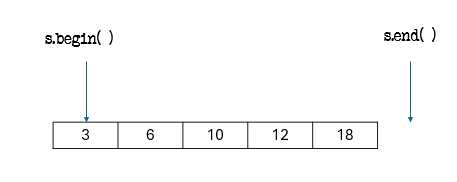
\includegraphics[width=0.6\textwidth]{immagini/2 - Strutture Dati/Set/set.png}
	\caption{Rappresentazione grafica di un \textbf{set}}
	\label{fig:strutture-dati:set}
\end{figure}


\subsection{Dichiarazione di un set}

\begin{lstlisting}[language=C++]
	#include <set>
	#include <iostream>
	using namespace std;
	
	set<int> s1;             // set vuoto di interi
	
	set<int> s2 = {5, 1, 9, 1, 3};  // inizializzazione con duplicati
	// Risultato: {1, 3, 5, 9}  (gli elementi duplicati vengono ignorati)
	
	set<string, greater<string>> s3 = {"mela", "pera", "banana"};
	// greater<string> ordina in modo decrescente
\end{lstlisting}

\textbf{Note:}
\begin{itemize}
	\item Gli elementi di un set sono sempre univoci.
	\item La struttura mantiene automaticamente l’ordine.
	\item Se si vuole un set non ordinato, si può usare \texttt{unordered\_set}.
\end{itemize}

\subsection{Operazioni principali sui set}

Le operazioni che seguono fanno riferimento al set della figura \ref{fig:strutture-dati:set}.

\begin{itemize}
	
	\item \textbf{Inserimento di un elemento:} \texttt{s.insert(valore)}
	\begin{lstlisting}[language=C++]
		s.insert(4);     // inserisce l'elemento 4
		s.insert(3);     // ignorato se 3 e' gia' presente
	\end{lstlisting}
	Complessità: O(log n)
	
	\item \textbf{Rimozione di un elemento:} \texttt{s.erase(valore)}
	\begin{lstlisting}[language=C++]
		s.erase(1);      // rimuove l'elemento 1 se presente
	\end{lstlisting}
	Complessità: O(log n)
	
	\item \textbf{Ricerca di un elemento:} \texttt{s.find(valore)}
	\begin{lstlisting}[language=C++]
		auto it = s.find(3);
		if (it != s.end())
		cout << "Trovato: " << *it;
		else
		cout << "Elemento non trovato";
	\end{lstlisting}
	Complessità: O(log n)
	
	\item \textbf{Verifica esistenza di un elemento:} \texttt{s.count(valore)}
	\begin{lstlisting}[language=C++]
		if (s.count(5)) cout << "Presente!";
		else cout << "Assente!";
	\end{lstlisting}
	Restituisce 1 se l’elemento esiste, 0 altrimenti.  
	Complessità: O(log n)
	
	\item \textbf{Dimensione:} \texttt{s.size()}
	\begin{lstlisting}[language=C++]
		cout << s.size();   // numero di elementi nel set
	\end{lstlisting}
	Complessità: O(1)
	
	\item \textbf{Controllo se vuoto:} \texttt{s.empty()}
	\begin{lstlisting}[language=C++]
		if (s.empty()) cout << "Set vuoto";
	\end{lstlisting}
	Complessità: O(1)
\end{itemize}

	\item \textbf{Accesso ad un elemento:}
	
	L'accesso ad un elemento di un \textbf{set} avviene mediante dereferenziazione dell'iteratore. 
	
	Questa volta però, a differenza dei \texttt{vector}, non possiamo accedere ad un elemento sommando un intero all'iteratore:
	
	\begin{lstlisting}[language=C++]
		#include <iostream>
		#include <set>
		using namespace std;
		
		int main() {
			set<int> s = {1, 3, 5, 7};
			
			it = s.begin();   
			
			// voglio stampare il 4 elemento
			cout << s.begin() + 3; // stampa un errore!
			
			return 0;
		}
		
	\end{lstlisting}
	
	L'errore è dovuto al fatto che gli iteratori dei set non supportano l'aritmetica dei puntatori. Possiamo solo avanzare o retrocedere di una posizione alla volta (con \texttt{it++} e \texttt{it---}).
	
	Quindi se volessi accedere al terzo elemento, una soluzione potrebbe essere:
	
	
	\begin{lstlisting}[language=C++]
		#include <iostream>
		#include <set>
		using namespace std;
		
		int main() {
			set<int> s = {1, 3, 5, 7};
			
			it = s.begin();  
			
			it++;
			it++; 
			
			// Attenzione: fare it = it + 2 è errato in quanto gli iteratori dei set non supportano l'aritmetica dei puntatori!
			
			cout << *it; // Stampa 5
			
			return 0;
		}
		
	\end{lstlisting}
	
		Un’alternativa è utilizzare la libreria \texttt{<iterator>}, che mette a disposizione la funzione \textbf{advance(iteratore, n)}.
		Questa funzione permette di spostare l’iteratore di \texttt{n} posizioni lungo il contenitore.
		
		È doveroso notare che la funzione \texttt{advance(valore, n)} può andare ben oltre la posizione \texttt{s.end( )}. Ciò significa che è opportuno verificare che il set abbia elementi sufficienti per accedere alla posizione desiderata:
		
		\begin{lstlisting}[language=C++]
			#include <iostream>
			#include <set>
			#include <iterator>
			using namespace std;
			
			int main() {
				set<int> s = {1, 3, 5, 7, 9};
				
				// controlliamo prima che il set abbia almeno 3 elementi
				if (s.size() >= 3) {
					auto it = s.begin();     // iteratore all'inizio
					advance(it, 2);          // spostiamo l'iteratore di 2 posizioni (3° elemento)
					cout << "Il terzo elemento e': " << *it << endl;
				} else {
					cout << "Il set ha meno di 3 elementi." << endl;
				}
				
				return 0;
			}
			
		\end{lstlisting}

		
	
	
\newpage
	
	
\subsection{Altre operazioni utili}

\begin{itemize}
	\item \textbf{lower\_bound}
	
	Restituisce un iteratore al primo elemento \textbf{maggiore o uguale} al valore passato come parametro.
	Restituisce \texttt{s.end( )} se non trova nulla.
	
	\begin{lstlisting}[language=C++]
		#include <iostream>
		#include <set>
		using namespace std;
		
		int main() {
			set<int> s = {1, 3, 5, 7};
			
			auto it = s.lower_bound(3); // primo elemento >= 3
			if(it != s.end())
			cout << "lower_bound(3) = " << *it << endl;
			
			return 0;
		}
	\end{lstlisting}
	
	Output: \texttt{lower\_bound(3) = 3}
	
	\item \textbf{upper\_bound}
	
	Restituisce un iteratore al primo elemento \textbf{maggiore} del valore passato come parametro.
	\textbf{s.end( )} se non trova nulla.
	
	\begin{lstlisting}[language=C++]
		#include <iostream>
		#include <set>
		using namespace std;
		
		int main() {
			set<int> s = {1, 3, 5, 7};
			
			auto it = s.upper_bound(3); // primo elemento > 3
			if(it != s.end())
			cout << "upper_bound(3) = " << *it << endl;
			
			return 0;
		}
	\end{lstlisting}
	
	Output: \texttt{upper\_bound(3) = 5}
	
\end{itemize}
	
\newpage
\subsection{Iterazione su un set}

\begin{lstlisting}[language=C++]
	for (auto it = s.begin(); it != s.end(); ++it)
	cout << *it << " ";
	
	// range-based for (C++11+)
	for (auto x : s)
	cout << x << " ";
\end{lstlisting}

\textbf{Note:}
\begin{itemize}
	\item L’iteratore restituisce il valore direttamente, non una coppia chiave-valore.
	\item Gli elementi sono ordinati automaticamente.
\end{itemize}


\subsection{Esempio pratico}

\begin{lstlisting}[language=C++]
	#include <set>
	#include <iostream>
	using namespace std;
	
	int main() {
		set<int> s;
		
		s.insert(10);
		s.insert(5);
		s.insert(10);
		s.insert(8);
		
		cout << "Elementi nel set: ";
		for (int x : s) cout << x << " ";
		
		cout << "\nDimensione: " << s.size() << endl;
		
		if (s.find(5) != s.end())
		cout << "5 e' presente!\n";
		
		s.erase(8);
		cout << "Dopo cancellazione: ";
		for (int x : s) cout << x << " ";
		
		return 0;
	}
\end{lstlisting}

\textbf{Output:}
\begin{verbatim}
	Elementi nel set: 5 8 10
	Dimensione: 3
	5 e' presente!
	Dopo cancellazione: 5 10
\end{verbatim}

\newpage

\subsection{Complessità computazionale riassunta}

In tabella \ref{tab:strutture-dati:set:complessita} sono state riassute le complessità computazionali delle operazione sui \textbf{set}\footnote{La funzione \texttt{advance(it, n)} ha complessità \texttt{O(n)}}

\begin{table}[h!]
	\centering
	\renewcommand{\arraystretch}{1.5}
	\setlength{\tabcolsep}{12pt}
	\begin{tabular}{|c|c|}
		\hline
		\textbf{Operazione} & \textbf{Complessità} \\
		\hline
		\makecell{Inserimento \\ \texttt{s.insert(x)}} & O(log n) \\
		\hline
		\makecell{Ricerca \\ \texttt{s.find(x)}} & O(log n) \\
		\hline
		\makecell{Cancellazione \\ \texttt{s.erase(x)}} & O(log n) \\
		\hline
		\makecell{Controllo esistenza \\ \texttt{s.count(x)}} & O(log n) \\
		\hline
		\makecell{lower\_bound \\ \texttt{s.lower\_bound(x)}} & O(log n) \\
		\hline
		\makecell{upper\_bound \\ \texttt{s.upper\_bound(x)}} & O(log n) \\
		\hline
		\makecell{Dimensione \\ \texttt{s.size()}} & O(1) \\
		\hline
		\makecell{Controllo se vuoto \\ \texttt{s.empty()}} & O(1) \\
		\hline
	\end{tabular}
	\caption{Complessità operazioni principali sui set}
	\label{tab:strutture-dati:set:complessita}
	
\end{table}




\newpage
\section{Multiset}


Il \textbf{multiset} è una struttura dati della libreria standard di C++ molto simile al \texttt{set}, con una differenza fondamentale: 
mentre nel \texttt{set} ogni elemento è unico, nel \texttt{multiset} possono esistere più copie dello stesso valore.

\begin{lstlisting}[language=C++]
	#include <iostream>
	#include <set>
	using namespace std;
	
	int main() {
		multiset<int> ms;
		ms.insert(5);
		ms.insert(5);
		ms.insert(3);
		ms.insert(7);
		
		for (int x : ms)
		cout << x << " "; // stampa: 3 5 5 7
	}
\end{lstlisting}

Come il \texttt{set}, anche il \texttt{multiset} memorizza gli elementi in modo ordinato e permette di eseguire operazioni 
di inserimento, ricerca e cancellazione in \texttt{O(log n)}.

\subsection{Caratteristiche principali}
\begin{itemize}
	\item Gli elementi sono \textbf{ordinati automaticamente}.
	\item È possibile inserire \textbf{valori duplicati}.
	\item Non è possibile accedere agli elementi tramite indice.
	\item Gli iteratori sono bidirezionali, quindi non supportano operazioni aritmetiche (\texttt{it + n}).
\end{itemize}


\subsection{Esempio pratico}

\begin{lstlisting}[language=C++]
	#include <iostream>
	#include <set>
	using namespace std;
	
	int main() {
		multiset<int> ms = {2, 3, 3, 5, 5, 5};
		
		cout << "Numero di 5: " << ms.count(5) << endl; // 3
		
		ms.erase(ms.find(3)); // cancella solo una delle due occorrenze di 3
		
		for (int x : ms)
		cout << x << " "; // stampa: 2 3 5 5 5
	}
\end{lstlisting}

\newpage
\subsection{Complessità computazionale riassunta}


\begin{table}[h!]
	\centering
	\renewcommand{\arraystretch}{1.5}
	\setlength{\tabcolsep}{12pt}
	\begin{tabular}{|c|c|}
		\hline
		\textbf{Operazione} & \textbf{Complessità} \\
		\hline
		\makecell{Inserimento \\ \texttt{ms.insert(x)}} & O(log n) \\
		\hline
		\makecell{Ricerca \\ \texttt{ms.find(x)}} & O(log n) \\
		\hline
		\makecell{Cancellazione di un elemento \\ \texttt{ms.erase(it)}} & O(1) \\
		\hline
		\makecell{Cancellazione di tutti gli elementi con un certo valore \\ \texttt{ms.erase(x)}} & O(log n + k)\footnotemark \\ 
		\hline
		\makecell{Conteggio occorrenze \\ \texttt{ms.count(x)}} & O(log n + k) \\
		\hline
		\makecell{lower\_bound \\ \texttt{ms.lower\_bound(x)}} & O(log n) \\
		\hline
		\makecell{upper\_bound \\ \texttt{ms.upper\_bound(x)}} & O(log n) \\
		\hline
		\makecell{Dimensione \\ \texttt{ms.size()}} & O(1) \\
		\hline
		\makecell{Controllo se vuoto \\ \texttt{ms.empty()}} & O(1) \\
		\hline
	\end{tabular}
	\caption{Complessità operazioni principali sui multiset}
\end{table}

\footnotetext{Nella tabella delle complessità del multiset, la lettera \texttt{k} indica il numero di elementi con lo stesso valore (cioè il numero di duplicati). Infatti \texttt{ms.erase(x)} deve cancellare k occorrenze e, di conseguenza, la complessità risulta \texttt{O(log n)} per la ricerca più \texttt{k} per eliminare ogni occorenza )}





\newpage

\section{Stack}


Lo \textbf{stack} (in italiano: pila) è una struttura dati della Standard Template Library (STL) che segue il principio \textbf{LIFO} (\textit{Last In, First Out}), ovvero l’ultimo elemento inserito è il primo a essere rimosso.

In figura \ref{fig:strutture-dati:stack} è mostrata la logica di funzionamento di una pila:  
gli elementi vengono aggiunti (push) e rimossi (pop) sempre dalla stessa estremità.

\begin{figure}[h!]
	\centering
	
\includegraphics[width=0.5\textwidth]{immagini/2 - Strutture Dati/Stack/stack.png}
	\caption{Rappresentazione grafica di uno \textbf{stack}}
	\label{fig:strutture-dati:stack}
\end{figure}

\subsection{Dichiarazione di uno stack}

\begin{lstlisting}[language=C++]
	#include <stack>
	#include <iostream>
	using namespace std;
	
	int main() {
		stack<int> s;     // dichiara uno stack di interi vuoto
		
		s.push(10);       // inserisce 10
		s.push(20);       // inserisce 20
		s.push(30);       // inserisce 30
		
		cout << "Top: " << s.top() << endl; // stampa 30
		
		s.pop();          // rimuove l'ultimo elemento inserito (30)
		
		cout << "Top dopo pop: " << s.top() << endl; // stampa 20
	}
\end{lstlisting}

\textbf{Note:}
\begin{itemize}
	\item Lo stack non consente accesso diretto agli elementi (come con gli indici).
	\item È possibile accedere solo all’elemento in cima (\texttt{top()}).
	\item La classe \texttt{stack} è un \textit{adattatore di contenitore}, che di default usa un \texttt{deque} come contenitore sottostante.
\end{itemize}

\subsection{Operazioni principali sullo stack}

Le operazioni principali disponibili sono:

\begin{itemize}
	\item \textbf{push(valore)} – Inserisce un nuovo elemento in cima alla pila.
	\begin{lstlisting}[language=C++]
		s.push(42);
	\end{lstlisting}
	Complessità: O(1)
	
	\item \textbf{pop()} – Rimuove l’elemento in cima alla pila.
	\begin{lstlisting}[language=C++]
		s.pop();
	\end{lstlisting}
	Complessità: O(1)
	
	\item \textbf{top()} – Restituisce una \textbf{riferimento} all’elemento in cima.
	\begin{lstlisting}[language=C++]
		cout << s.top();
	\end{lstlisting}
	Complessità: O(1)
	
	\item \textbf{empty()} – Verifica se la pila è vuota.
	\begin{lstlisting}[language=C++]
		if (s.empty()) cout << "Stack vuoto!";
	\end{lstlisting}
	Complessità: O(1)
	
	\item \textbf{size()} – Restituisce il numero di elementi presenti nello stack.
	\begin{lstlisting}[language=C++]
		cout << s.size();
	\end{lstlisting}
	Complessità: O(1)
\end{itemize}

\subsection{Iterazione su uno stack}

Lo \texttt{stack} \textbf{non supporta l’iterazione diretta} (come con \texttt{for(auto x : s)} o iteratori), poiché è pensato per un accesso controllato di tipo LIFO.  
Tuttavia, è possibile svuotarlo progressivamente per leggere tutti i suoi elementi:

\begin{lstlisting}[language=C++]
	#include <stack>
	#include <iostream>
	using namespace std;
	
	int main() {
		stack<int> s;
		s.push(10);
		s.push(20);
		s.push(30);
		
		while (!s.empty()) {
			cout << s.top() << " ";
			s.pop();
		}
		// Output: 30 20 10
	}
\end{lstlisting}

\textbf{Nota:}  
Questo metodo svuota lo stack. Se serve mantenerlo, conviene copiarlo prima in un altro stack.

\subsection{Esempio pratico}

\begin{lstlisting}[language=C++]
	#include <stack>
	#include <iostream>
	using namespace std;
	
	int main() {
		stack<string> history;
		
		history.push("www.google.com");
		history.push("www.openai.com");
		history.push("www.github.com");
		
		cout << "Pagina corrente: " << history.top() << endl;
		history.pop();
		
		cout << "Torno a: " << history.top() << endl;
		
		cout << "Totale pagine: " << history.size() << endl;
	}
\end{lstlisting}

\textbf{Output:}
\begin{verbatim}
	Pagina corrente: www.github.com
	Torno a: www.openai.com
	Totale pagine: 2
\end{verbatim}

\subsection{Complessità computazionale riassunta}

\begin{table}[h!]
	\centering
	\renewcommand{\arraystretch}{1.5}
	\setlength{\tabcolsep}{12pt}
	\begin{tabular}{|c|c|}
		\hline
		\textbf{Operazione} & \textbf{Complessità} \\
		\hline
		\makecell{Inserimento \\ \texttt{s.push(x)}} & O(1) \\
		\hline
		\makecell{Rimozione \\ \texttt{s.pop()}} & O(1) \\
		\hline
		\makecell{Accesso al top \\ \texttt{s.top()}} & O(1) \\
		\hline
		\makecell{Controllo se vuoto \\ \texttt{s.empty()}} & O(1) \\
		\hline
		\makecell{Dimensione \\ \texttt{s.size()}} & O(1) \\
		\hline
	\end{tabular}
	\caption{Complessità operazioni principali sullo stack}
	\label{tab:strutture-dati:stack:complessita}
\end{table}





\newpage

\section{Queue}

La \textbf{queue} (in italiano: coda) è una struttura dati della STL che segue il principio \textbf{FIFO} (\textit{First In, First Out}), ovvero il primo elemento inserito è il primo a essere rimosso.  
Si comporta come una vera e propria coda di persone: chi entra per primo esce per primo.

Di fatto è il contrario di uno \texttt{stack}

In figura \ref{fig:strutture-dati:queue} è illustrato il funzionamento logico della coda.

\begin{figure}[h!]
	\centering
	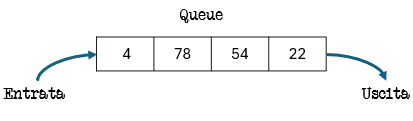
\includegraphics[width=0.6\textwidth]{immagini/2 - Strutture Dati/queue/queue.png}
	\caption{Rappresentazione grafica di una \textbf{queue}}
	\label{fig:strutture-dati:queue}
\end{figure}

\subsection{Dichiarazione di una queue}

\begin{lstlisting}[language=C++]
	#include <queue>
	#include <iostream>
	using namespace std;
	
	int main() {
		queue<int> q;      // dichiara una coda di interi
		
		q.push(10);        // inserisce 10 in fondo alla coda
		q.push(20);        // inserisce 20
		q.push(30);        // inserisce 30
		
		cout << "Front: " << q.front() << endl; // stampa 10
		cout << "Back: " << q.back() << endl;   // stampa 30
		
		q.pop();          // rimuove il primo elemento (10)
		
		cout << "Front dopo pop: " << q.front() << endl; // stampa 20
	}
\end{lstlisting}

\textbf{Note:}
\begin{itemize}
	\item È possibile accedere solo all’elemento \textbf{front} (testa) e a quello \textbf{back} (coda).
	\item Non è possibile accedere direttamente agli elementi centrali o iterare sulla coda.
	\item Internamente, la \texttt{queue} è un \textbf{adattatore di contenitore}, che usa di default un \texttt{deque}.
\end{itemize}

\subsection{Operazioni principali sulla queue}

\begin{itemize}
	\item \textbf{push(valore)} – Inserisce un elemento in fondo alla coda.
	\begin{lstlisting}[language=C++]
		q.push(42);
	\end{lstlisting}
	Complessità: O(1)
	
	\item \textbf{pop()} – Rimuove l’elemento in testa alla coda.
	\begin{lstlisting}[language=C++]
		q.pop();
	\end{lstlisting}
	Complessità: O(1)
	
	\item \textbf{front()} – Restituisce una \textbf{riferimento} all’elemento in testa.
	\begin{lstlisting}[language=C++]
		cout << q.front();
	\end{lstlisting}
	Complessità: O(1)
	
	\item \textbf{back()} – Restituisce una \textbf{riferimento} all’ultimo elemento inserito.
	\begin{lstlisting}[language=C++]
		cout << q.back();
	\end{lstlisting}
	Complessità: O(1)
	
	\item \textbf{empty()} – Verifica se la coda è vuota.
	\begin{lstlisting}[language=C++]
		if (q.empty()) cout << "Coda vuota!";
	\end{lstlisting}
	Complessità: O(1)
	
	\item \textbf{size()} – Restituisce il numero di elementi nella coda.
	\begin{lstlisting}[language=C++]
		cout << q.size();
	\end{lstlisting}
	Complessità: O(1)
\end{itemize}

\subsection{Iterazione su una queue}

Come lo \texttt{stack}, anche la \texttt{queue} non supporta iteratori né accesso diretto.  
È possibile tuttavia svuotarla per leggere i valori in ordine di inserimento:

\begin{lstlisting}[language=C++]
	#include <queue>
	#include <iostream>
	using namespace std;
	
	int main() {
		queue<int> q;
		q.push(10);
		q.push(20);
		q.push(30);
		
		while (!q.empty()) {
			cout << q.front() << " ";
			q.pop();
		}
		// Output: 10 20 30
	}
\end{lstlisting}

\textbf{Nota:}  
Questo metodo svuota la coda. Se serve mantenere i dati, conviene copiarla prima in un’altra \texttt{queue}.

\subsection{Esempio pratico}

\begin{lstlisting}[language=C++]
	#include <queue>
	#include <iostream>
	using namespace std;
	
	int main() {
		queue<string> clienti;
		
		clienti.push("Marco");
		clienti.push("Giulia");
		clienti.push("Antonio");
		
		cout << "Serve: " << clienti.front() << endl;
		clienti.pop();
		
		cout << "Prossimo cliente: " << clienti.front() << endl;
		cout << "Ultimo in coda: " << clienti.back() << endl;
	}
\end{lstlisting}

\textbf{Output:}
\begin{verbatim}
	Serve: Marco
	Prossimo cliente: Giulia
	Ultimo in coda: Antonio
\end{verbatim}

\subsection{Complessità computazionale riassunta}

\begin{table}[h!]
	\centering
	\renewcommand{\arraystretch}{1.5}
	\setlength{\tabcolsep}{12pt}
	\begin{tabular}{|c|c|}
		\hline
		\textbf{Operazione} & \textbf{Complessità} \\
		\hline
		\makecell{Inserimento in coda \\ \texttt{q.push(x)}} & O(1) \\
		\hline
		\makecell{Rimozione in testa \\ \texttt{q.pop()}} & O(1) \\
		\hline
		\makecell{Accesso al primo elemento \\ \texttt{q.front()}} & O(1) \\
		\hline
		\makecell{Accesso all'ultimo elemento \\ \texttt{q.back()}} & O(1) \\
		\hline
		\makecell{Controllo se vuota \\ \texttt{q.empty()}} & O(1) \\
		\hline
		\makecell{Dimensione \\ \texttt{q.size()}} & O(1) \\
		\hline
	\end{tabular}
	\caption{Complessità operazioni principali sulla queue}
	\label{tab:strutture-dati:queue:complessita}
\end{table}





\newpage

\section{Priority Queue}

La \textbf{priority\_queue} è una struttura dati della STL che memorizza gli elementi secondo una \textbf{priorità}.  
A differenza della \texttt{queue} tradizionale, non segue l’ordine FIFO, ma estrae sempre l’elemento con la priorità più alta (di default il valore massimo).

\begin{figure}[h!]
	\centering
	\includegraphics[width=0.6\textwidth]{immagini/2 - Strutture Dati/PriorityQueue/priority_queue.png}
	\caption{Rappresentazione grafica di una \textbf{priority\_queue}}
	\label{fig:strutture-dati:priority_queue}
\end{figure}

\subsection{Dichiarazione di una priority\_queue}

\begin{lstlisting}[language=C++]
	#include <queue>
	#include <iostream>
	using namespace std;
	
	int main() {
		priority_queue<int> pq; // priority_queue di interi (max-heap)
		
		pq.push(10);
		pq.push(5);
		pq.push(20);
		
		cout << "Elemento con priorità massima: " << pq.top() << endl; // 20
		
		priority_queue<string> pq2;
		
		pq2.push("banana");
		pq2.push("mela");
		pq2.push("arancia");
		
		cout << "Massimo: " << pq2.top() << endl; 
		// stampa mela in quanto mela è considerata massima. Confrontando le stringhe alfabeticamente, viene dopo banana e arancia.
		
	}
\end{lstlisting}

\textbf{Note:}
\begin{itemize}
	\item Gli elementi sono ordinati automaticamente in base alla priorità.
	\item Di default è una \textbf{max-heap} (massimo elemento in cima).
	\item Per creare una \textbf{min-heap} si usa:
	\begin{lstlisting}[language=C++]
		priority_queue<int, vector<int>, greater<int>> pq_min;
	\end{lstlisting}
	
\end{itemize}

\subsection{Operazioni principali sulla priority\_queue}

\begin{itemize}
	\item \textbf{push(valore)} – Inserisce un elemento nella coda di priorità.
	\begin{lstlisting}[language=C++]
		pq.push(42);
	\end{lstlisting}
	Complessità: O(log n)
	
	\item \textbf{pop()} – Rimuove l’elemento con priorità più alta.
	\begin{lstlisting}[language=C++]
		pq.pop();
	\end{lstlisting}
	Complessità: O(log n)
	
	\item \textbf{top()} – Restituisce un riferimento all’elemento con priorità più alta.
	\begin{lstlisting}[language=C++]
		cout << pq.top();
	\end{lstlisting}
	Complessità: O(1)
	
	\item \textbf{empty()} – Verifica se la coda è vuota.
	\begin{lstlisting}[language=C++]
		if (pq.empty()) cout << "Priority queue vuota!";
	\end{lstlisting}
	Complessità: O(1)
	
	\item \textbf{size()} – Restituisce il numero di elementi presenti.
	\begin{lstlisting}[language=C++]
		cout << pq.size();
	\end{lstlisting}
	Complessità: O(1)
\end{itemize}

\subsection{Iterazione su una priority\_queue}
Così come la queue, non è possibile iterare direttamente o accedere agli elementi centrali.


\subsection{Esempio pratico}

\begin{lstlisting}[language=C++]
	#include <queue>
	#include <iostream>
	using namespace std;
	
	int main() {
		priority_queue<int> pq;
		
		pq.push(15);
		pq.push(30);
		pq.push(10);
		
		cout << "Massimo elemento: " << pq.top() << endl; // 30
		pq.pop();
		
		cout << "Nuovo massimo: " << pq.top() << endl;   // 15
		cout << "Dimensione: " << pq.size() << endl;     // 2
	}
\end{lstlisting}

\textbf{Output:}
\begin{verbatim}
	Massimo elemento: 30
	Nuovo massimo: 15
	Dimensione: 2
\end{verbatim}

\subsection{Complessità computazionale riassunta}

\begin{table}[h!]
	\centering
	\renewcommand{\arraystretch}{1.5}
	\setlength{\tabcolsep}{12pt}
	\begin{tabular}{|c|c|}
		\hline
		\textbf{Operazione} & \textbf{Complessità} \\
		\hline
		\makecell{Inserimento \\ \texttt{pq.push(x)}} & O(log n) \\
		\hline
		\makecell{Rimozione del massimo \\ \texttt{pq.pop()}} & O(log n) \\
		\hline
		\makecell{Accesso al massimo \\ \texttt{pq.top()}} & O(1) \\
		\hline
		\makecell{Controllo se vuota \\ \texttt{pq.empty()}} & O(1) \\
		\hline
		\makecell{Dimensione \\ \texttt{pq.size()}} & O(1) \\
		\hline
	\end{tabular}
	\caption{Complessità operazioni principali sulla priority\_queue}
	\label{tab:strutture-dati:priority_queue:complessita}
\end{table}


\textbf{Nota:} la \texttt{priority\_queue} è molto efficiente quando in un insieme di dati dobbiamo accedere frequentemente all'elemento massimo. Se invece è necessario poter iterare sulla struttura o accedere ad elementi “centrali”, è più conveniente utilizzare un \texttt{multiset}.




\newpage
\section{Deque}

La \textbf{deque} (double-ended queue, coda a doppia estremità) è una struttura dati della STL che permette l'inserimento e la rimozione di elementi sia all'inizio sia alla fine del contenitore.  
Si comporta come una combinazione tra \texttt{vector} e \texttt{queue}: supporta accesso casuale agli elementi e operazioni efficienti alle estremità.

In figura \ref{fig:strutture-dati:deque} è illustrato il funzionamento logico di una \textbf{deque}.

\begin{figure}[h!]
	\centering
	
\includegraphics[width=0.6\textwidth]{immagini/2 - Strutture Dati/Deque/deque.png}
	\caption{Rappresentazione grafica di una \textbf{deque}}
	\label{fig:strutture-dati:deque}
\end{figure}

\subsection{Dichiarazione di una deque}

\begin{lstlisting}[language=C++]
	#include <deque>
	#include <iostream>
	using namespace std;
	
	int main() {
		deque<int> d;             // deque vuota di interi
		
		d.push_back(10);          // inserisce 10 in coda
		d.push_front(5);          // inserisce 5 in testa
		d.push_back(20);          // inserisce 20 in coda
		
		cout << "Front: " << d.front() << endl; // stampa 5
		cout << "Back: " << d.back() << endl;   // stampa 20
	}
\end{lstlisting}

\textbf{Note:}
\begin{itemize}
	\item La \texttt{deque} permette inserimenti e cancellazioni sia in testa sia in coda in tempo costante O(1).
	\item Supporta accesso casuale agli elementi tramite l'operatore \texttt{[]}, come un \texttt{vector}.
	\item È più flessibile di un \texttt{queue} o \texttt{stack} perché consente operazioni su entrambe le estremità.
\end{itemize}

\subsection{Operazioni principali sulla deque}

\begin{itemize}
	\item \textbf{push\_front(valore)} – Inserisce un elemento all’inizio.
	\begin{lstlisting}[language=C++]
		d.push_front(3);
	\end{lstlisting}
	Complessità: O(1)
	
	\item \textbf{push\_back(valore)} – Inserisce un elemento alla fine.
	\begin{lstlisting}[language=C++]
		d.push_back(7);
	\end{lstlisting}
	Complessità: O(1)
	
	\item \textbf{pop\_front()} – Rimuove l’elemento in testa.
	\begin{lstlisting}[language=C++]
		d.pop_front();
	\end{lstlisting}
	Complessità: O(1)
	
	\item \textbf{pop\_back()} – Rimuove l’elemento in coda.
	\begin{lstlisting}[language=C++]
		d.pop_back();
	\end{lstlisting}
	Complessità: O(1)
	
	\item \textbf{front()} – Restituisce riferimento al primo elemento.
	\begin{lstlisting}[language=C++]
		cout << d.front();
	\end{lstlisting}
	Complessità: O(1)
	
	\item \textbf{back()} – Restituisce riferimento all’ultimo elemento.
	\begin{lstlisting}[language=C++]
		cout << d.back();
	\end{lstlisting}
	Complessità: O(1)
	
	\item \textbf{operator[]} – Accesso casuale ad un elemento.
	\begin{lstlisting}[language=C++]
		cout << d[1]; // secondo elemento
	\end{lstlisting}
	Complessità: O(1)
	
	\item \textbf{size()} – Numero di elementi.
	\begin{lstlisting}[language=C++]
		cout << d.size();
	\end{lstlisting}
	Complessità: O(1)
	
	\item \textbf{empty()} – Verifica se la deque è vuota.
	\begin{lstlisting}[language=C++]
		if(d.empty()) cout << "Deque vuota!";
	\end{lstlisting}
	Complessità: O(1)
\end{itemize}

\subsection{Iterazione su una deque}

\begin{lstlisting}[language=C++]
	for(auto it = d.begin(); it != d.end(); ++it)
	cout << *it << " ";
	
	// oppure con range-based for
	for(int x : d)
	cout << x << " ";
\end{lstlisting}

\subsection{Esempio pratico}

\begin{lstlisting}[language=C++]
	#include <deque>
	#include <iostream>
	using namespace std;
	
	int main() {
		deque<int> d;
		
		d.push_back(10);
		d.push_front(5);
		d.push_back(20);
		
		cout << "Elementi nella deque: ";
		for(int x : d) cout << x << " ";
		
		d.pop_front();
		cout << "\nDopo pop_front: ";
		for(int x : d) cout << x << " ";
		
		d.pop_back();
		cout << "\nDopo pop_back: ";
		for(int x : d) cout << x << " ";
		
		return 0;
	}
\end{lstlisting}

\textbf{Output:}
\begin{verbatim}
	Elementi nella deque: 5 10 20
	Dopo pop_front: 10 20
	Dopo pop_back: 10
\end{verbatim}


\newpage
\subsection{Complessità computazionale riassunta}

\begin{table}[h!]
	\centering
	\renewcommand{\arraystretch}{1.5}
	\setlength{\tabcolsep}{12pt}
	\begin{tabular}{|c|c|}
		\hline
		\textbf{Operazione} & \textbf{Complessità} \\
		\hline
		\makecell{Inserimento in testa \\ \texttt{push\_front(x)}} & O(1) \\
		\hline
		\makecell{Inserimento in coda \\ \texttt{push\_back(x)}} & O(1) \\
		\hline
		\makecell{Rimozione in testa \\ \texttt{pop\_front()}} & O(1) \\
		\hline
		\makecell{Rimozione in coda \\ \texttt{pop\_back()}} & O(1) \\
		\hline
		\makecell{Accesso al primo elemento \\ \texttt{front()}} & O(1) \\
		\hline
		\makecell{Accesso all'ultimo elemento \\ \texttt{back()}} & O(1) \\
		\hline
		\makecell{Accesso casuale \\ \texttt{operator[]}} & O(1) \\
		\hline
		\makecell{Controllo se vuota \\ \texttt{empty()}} & O(1) \\
		\hline
		\makecell{Dimensione \\ \texttt{size()}} & O(1) \\
		\hline
	\end{tabular}
	\caption{Complessità operazioni principali sulla deque}
	\label{tab:strutture-dati:deque:complessita}
\end{table}

\subsection{Differenze tra \texttt{queue} e \texttt{deque}}

A questo punto potremmo chiederci perché usare una \texttt{queue} quando abbiamo a disposizione la \texttt{deque} che, effettivamente, fa più cose senza aumentare la complessità computazionale.

La differenza principale tra \texttt{queue} e \texttt{deque}, aldilà delle funzionalità base, sta nel tipo di astrazione che vogliamo utilizzare.

\begin{itemize}
	\item \textbf{\texttt{queue}}
	\begin{itemize}
		\item È un \textbf{adattatore di contenitore}: ci interessa solo il comportamento FIFO.
		\item Non permette l'accesso agli elementi centrali né l'iterazione.
		\item L'interfaccia è semplice: \texttt{push}, \texttt{pop}, \texttt{front}, \texttt{back}.
		\item Vantaggio: garantisce \textbf{chiarezza e sicurezza}, perché chi legge il codice sa subito che si sta usando una coda "pura".
	\end{itemize}
	
	\item \textbf{\texttt{deque}}
	\begin{itemize}
		\item È un \textbf{contenitore generico}: permette quasi tutte le operazioni, come iterazione, accesso casuale, inserimenti/rimozioni sia in testa che in coda.
		\item Offre più flessibilità, ma anche più possibilità di usare la struttura in modo non coerente con una coda FIFO.
	\end{itemize}
\end{itemize}

In pratica:
\begin{itemize}
	\item Se vogliamo solo una coda, usiamo \texttt{queue}: comunica chiaramente l'intento e riduce il rischio di errori.
	\item Se vogliamo più flessibilità (accesso casuale, iterazione, manipolazioni complesse), usiamo \texttt{deque}.
\end{itemize}

\textit{È come scegliere tra un coltellino e un coltellino svizzero: il coltellino fa una cosa e la fa bene, il coltellino può fare di più ma non sempre è la scelta più chiara.}


